%%%%%%%%%%%%%%
% LECTURE 10 %
%%%%%%%%%%%%%%
\vspace{1cm}
\noindent\lecture{10}{08/11/2021}
\vspace{0.5cm}

\section{Interazione con l'ambiente}
Focalizziamo la nostra attenzione sul discorso riguardante i qubit e sul modo con cui interagiscono con l'ambiente in cui sono immersi, ossia come sono influenzati dal rumore, dalla temperatura, ecc. Lo spazio di Hilbert generale è il prodotto tensoriale tra quello del qubit e quello dell'ambiente: $\mathcal{H} = \mathcal{H}_q \otimes \mathcal{H}_E$ (pedice $E$ per "environment"). Come visto dai postulati della QM, possiamo assumere che l'evoluzione temporale in $\mathcal{H}$ sia unitaria: se assumiamo uno stato puro iniziale $\ket{\psi} \in \mathcal{H}$, allora esso evolverà in $\ket{\psi}' = U \ket{\psi}$ dove $U$ è un operatore unitario. 

\noindent Come evidenziato nella sezione precedente, non vogliamo studiare il qubit mantenendo tutti i gradi di libertà dell'ambiente, quindi possiamo calcolare una traccia parziale su $\mathcal{H}_E$: si ricordi che anche se $\ket{\psi}$ è uno stato puro, alla fine otteniamo una matrice densità $\rho$ che descrive il sottosistema $\mathcal{H}_q$. Ad esempio, se il qubit è preparato nella sovrapposizione $\ket{\psi} = a \ket{0} + b \ket{1}$, dal punto di vista della fisica del qubit esso si trova in uno stato puro; quando si considera tuttavia l'intero sistema costituito anche dall'ambiente, la traccia parziale su $\mathcal{H}_E$ produce una matrice densità del qubit tale che possa corrispondere ad una miscela di stati nonostante si partisse da uno stato puro!

\noindent Un punto importante da tenere sempre in considerazione è che l'evoluzione temporale del sottosistema del qubit non è necessariamente unitaria: supponiamo ad esempio che l'evoluzione di $\mathcal{H}$ sia descritta dal seguente circuito
\begin{center}
    \mbox{
        \Qcircuit @C=2em @R=1em {
            \lstick{\text{Qubit}} & \multigate{1}{U} & \gate{} & \rstick{\ket{\psi}} \qw \\
            \lstick{\text{Ambiente}} & \ghost{U} & \qw & \qw \gategroup{1}{3}{1}{3}{.7em}{--}
        }
    }
\end{center}
dove l'evoluzione totale $U$ è unitaria. Il problema è che il risultato $\ket{\psi} \in \mathcal{H}_q$ dell'evoluzione del qubit potrebbe derivare da un operatore non unitario di $\mathcal{H}_q$! (si veda il gate ignoto nel riquadro tratteggiato).
 
\noindent Uno dei modi per realizzare un qubit è quello di considerare un atomo che presenta due livelli energetici vicini tra loro, ma facilmente isolabili rispetto ai livelli restanti. Chiamiamo $\ket{1}$ e $\ket{0}$ lo stato eccitato e il ground state rispettivamente. Un fenomeno che accade spontaneamente in natura è l'\textbf{emissione spontanea} di fotoni
\begin{center}
    \mbox{
        \Qcircuit @C=2em @R=2em {
            & \qw & \rstick{\ket{1}} \qw \\
            & \raisebox{.3em}{\begin{huge}$\downarrow$\end{huge}} & \raisebox{.05em}{\begin{huge} $\rightsquigarrow$ \end{huge}}\\
            & \qw & \rstick{\ket{0}} \qw
        }
    }
\end{center}
\vspace{0.2cm}
(la freccia verticale indica la transizione $\ket{1} \rightarrow \ket{0}$, mentre quella orizzontale indica l'emissione del fotone). In generale questo accade sempre se si aspetta un tempo sufficientemente lungo. Chiaramente il fotone emesso viene perso nell'ambiente, quindi dal punto di vista del qubit, $\mathcal{H}_q$ è lo spazio di Hilbert dei livelli energetici, mentre la radiazione ambientale di background, che è parte del campo elettromagnetico quantizzato, costituisce l'ambiente in cui il qubit è immerso. Come detto sopra, dal punto di vista del sistema totale l'evoluzione è unitaria, tuttavia in $\mathcal{H}_q$ l'emissione spontanea è descritta dal seguente operatore $\tilde U$
\begin{equation*}
    \tilde U \, : \, 
    \begin{cases}
        \ket{1} \rightarrow \ket{0} \\
        \ket{0} \rightarrow \ket{0}
    \end{cases} \, , \quad \Rightarrow \quad 
    \tilde U = 
    \begin{pmatrix}
        0 & 1 \\ 0 & 0 
    \end{pmatrix} \, ,
\end{equation*}
e chiaramente la matrice $\tilde U$ non è unitaria!

\noindent Diamo uno sguardo più dettagliato a questi processi generali. Supponiamo che $\mathcal{H}$ sia un sistema \textbf{chiuso} descritto da un evoluzione unitaria $U$ tale che
\begin{align*}
    \ket{\psi} &\rightarrow U \ket{\psi} \, , \\
    \bra{\psi} &\rightarrow \bra{\psi} U^\dag \, ;
\end{align*}
usando il formalismo della matrice densità possiamo scrivere $\rho = \ketbra{\psi}$: come evolve $\rho$ a seguito di evoluzioni unitarie degli stati? Semplicemente
\begin{equation*}
    \rho = \ketbra{\psi} \rightarrow U \ketbra{\psi} U^\dag = U \rho \, U^\dag \, ,
\end{equation*}
quindi la matrice densità evolve per \textbf{coniugazione}. Questo vale anche nel caso di miscele, infatti
\begin{equation*}
    \rho = \sum_i \rho_i \ketbra{\psi_i} \rightarrow \sum_i \rho_i \, U \ketbra{\psi_i} U^\dag = U \rho \, U^\dag \, .
\end{equation*}
Ritorniamo al sistema totale descritto da $\tilde{\mathcal{H}} = \mathcal{H}_q \otimes \mathcal{H}_E$: chiamiamo $\tilde \rho$ la matrice densità totale di $\tilde{\mathcal{H}}$, la quale può descrivere sia stati puri sia miscele (in generale a seguito della presenza di una temperatura finita si parte sempre con una miscela di stati). Scriviamo $\tilde \rho = \rho \otimes \rho_E$, dove chiaramente $\rho$ è la matrice densità in $\mathcal{H}_q$. Cosa succede se si aspetta un tempo abbastanza lungo? Analizziamo la seguente situazione
\begin{center}
    \mbox{
        \Qcircuit @C=2em @R=1em {
            \lstick{\text{Qubit: } \; \rho} & \multigate{1}{U} & \gate{} & \rstick{\mathcal{E}(\rho)} \qw \\
            \lstick{\text{Ambiente: } \; \rho_E} & \ghost{U} & \qw & \qw \gategroup{1}{3}{1}{3}{.7em}{--}
        }
    }
\end{center}
dove $\mathcal{E}(\rho)$ è l'evoluto di $\rho$ in $\mathcal{H}_q$. Sappiamo che se il sistema totale qubit-ambiente è chiuso allora $\tilde \rho$ evolverà per coniugazione come $\tilde \rho \rightarrow U (\rho \otimes \rho_E) U^\dag$. Come al solito, per ignorare i gradi di libertà dell'ambiente prendiamo una traccia parziale su di esso: definiamo la matrice densità
\begin{equation}\label{evolution_rho_qubit}
    \mathcal{E}(\rho) = \Tr_E \left[ U (\rho \otimes \rho_E) U^\dag \right] \, ,
\end{equation}
che dà una descrizione efficace del qubit e ne descrive la fisica dal suo punto di vista. La mappa $\rho \rightarrow \mathcal{E}(\rho)$ non è unitaria in generale! Come possiamo caratterizzare l'evoluzione dal punto di vista del qubit? Abbiamo detto che
\begin{center}
    \mbox{
        $
        \begin{matrix}
             \\
             \\
            \Large\substack{\text{Sistema} \\ \text{completo}}: \\
        \end{matrix}
        $
        $
        \begin{matrix}
             \\
             \\
            \qquad \\
        \end{matrix}
        $
        $
        \begin{matrix}
             \\
             \\
            \qquad \\
        \end{matrix}
        $
        $
        \begin{matrix}
             \\
             \\
            \qquad \\
        \end{matrix}
        $
        \raisebox{-.95em}{
            \Qcircuit @C=1em @R=1em {
                \lstick{\tilde \rho} & \gate{U} & \rstick{U \tilde \rho \, U^\dag \; ,} \qw
            }
        }
    }
    \qquad \qquad \qquad
    \mbox{
        $
        \begin{matrix}
             \\
             \\
            \Large\substack{\text{Sistema} \\ \text{ridotto}}: \\
        \end{matrix}
        $
        $
        \begin{matrix}
             \\
             \\
            \qquad \\
        \end{matrix}
        $
        $
        \begin{matrix}
             \\
             \\
            \qquad \\
        \end{matrix}
        $
        $
        \begin{matrix}
             \\
             \\
            \qquad \\
        \end{matrix}
        $
        $
        \begin{matrix}
             \\
             \\
            \qquad \\
        \end{matrix}
        $
        $
        \begin{matrix}
             \\
             \\
            \qquad \\
        \end{matrix}
        $
        \Qcircuit @C=1em @R=1em {
            \lstick{\rho} & \multigate{1}{U} & \rstick{\mathcal{E}(\rho)} \qw \\
            \lstick{\rho_E} & \ghost{U} & \qw
        }
        \raisebox{-1.2em}{\qquad \quad ,}
    }
\end{center}
Supponiamo che $\mathcal{H}_E$ possieda la base $\{ \ket{e_k} \}$, allora la \eqref{evolution_rho_qubit} diventa 
\begin{equation*}
    \mathcal{E}(\rho) = \sum_k \expval{U (\rho \otimes \rho_E) U^\dag}{e_k} \, ,
\end{equation*}
dove sottolineiamo che la notazione non deve trarre in inganno perché $U$ e $U^\dag$ agiscono sia sul qubit sia sull'ambiente (il RHS rimane un operatore, non una somma di elementi di matrice). Supponiamo che l'ambiente sia in uno stato puro iniziale, che chiamiamo $\ket{e_0}$: possiamo sempre assumere questa condizione senza alcuna perdita di generalità grazie al teorema di purificazione; quindi $\rho_E = \ketbra{e_0}$. In questo modo la precedente diventa
\begin{equation*}
    \mathcal{E}(\rho) = \sum_k \mel{e_k}{U}{e_0} \rho \mel{e_0}{U^\dag}{e_k} \, ,
\end{equation*}
dove come prima notiamo che $\mel{e_k}{U}{e_0}$ e $\mel{e_0}{U^\dag}{e_k}$ non sono elementi di matrice ma rimangono operatori agenti sul qubit. Chiamiamo 
\begin{equation}\label{E_k}
    E_k \equiv \mel{e_k}{U}{e_0} \, ,
\end{equation}
questi operatori ottenuti come elementi di matrice parziali con $e_k$ e $e_0$: spesso vengono chiamati \textbf{operation elements}. In questo modo $\mathcal{E}(\rho)$ può essere scritto come
\begin{equation}\label{operator_sum_repr}
    \mathcal{E}(\rho) = \sum_k E_k \rho E_k^\dag \, ,
\end{equation}
il quale prende il nome di \textbf{operator-sum representation}; la mappa $\mathcal{E}(\rho)$, invece, prende il nome di \textbf{quantum operation}. Dato che $\mathcal{E}(\rho)$ è una matrice densità deve soddisfare la condizione $\Tr \mathcal{E}(\rho) = 1$:
\begin{equation*}
    \Tr \mathcal{E}(\rho) = \Tr \left( \sum_k E_k \rho E_k^\dag \right) = \sum_k \Tr \left( E_k \rho E_k^\dag \right) = \sum_k \Tr \left( \rho E_k^\dag E_k \right) \overset{!}{=} 1 \, ;
\end{equation*}
dove nell'ultimo passaggio abbiamo usato la proprietà ciclica della traccia. Dato che $\Tr \rho = 1$, allora gli operation elements devono soddisfare il vincolo seguente
\begin{equation}\label{constraint_E_k}
    \sum_k E_k^\dag E_k = \mathbb{I} \, .
\end{equation}
Notiamo che nella \eqref{constraint_E_k} si ha in generale $E^\dag_k E_k \neq \mathbb{I}$, quindi $E_k$ non sono unitari! 

\noindent Qual è l'interpretazione fisica della \eqref{operator_sum_repr}? Si assume che esistano numerosi processi, etichettati da $k$, ognuno dei quali è visto come un sottosistema in cui è eseguita una particolare evoluzione temporale, data da $\rho \rightarrow E_k \rho E_k^\dag$. Ancora una volta, non si tratta di una coniugazione perché gli $E_k$ non sono in generale unitari. Ciascun operatore $E_k$ descritto dalla \eqref{E_k} è visto come un salto degli stati dell'ambiente da $\ket{e_0}$ a $\ket{e_k}$. 

\noindent Cominciamo a capire meglio come l'ambiente interagisce con i qubit guardando degli esempi espliciti. Supponiamo un qubit nella sovrapposizione $a\ket{0} + b\ket{1}$ che interagisce con l'ambiente: gli stati possono essere invertiti, possono essere aggiunte delle fasi (cambiano i segni dei coefficienti) e più in generale i coefficienti stessi possono cambiare. Vediamo esplicitamente che cosa può succedere. 

\begin{esempio}[\textbf{Bit flip channel}]
    Il primo esempio che analizziamo è il caso in cui gli stati vengano invertiti: $\ket{0} \rightarrow \ket{1}$ e $\ket{1} \rightarrow \ket{0}$. Che cosa ci aspettiamo per gli operatori $E_k$? Chiaramente uno degli operatori può essere $X$, dato che agisce sui singoli qubit; tuttavia $X$ da solo non è sufficiente per soddisfare il vincolo \eqref{constraint_E_k}, quindi aggiungiamo anche l'identità: scriviamo
    \begin{equation*}
        E_0 = \sqrt{p} \, \mathbb{I} = \sqrt{p}
        \begin{pmatrix}
            1 & 0 \\ 0 & 1
        \end{pmatrix} \, , \qquad
        E_1 = \sqrt{1-p} X = \sqrt{1-p}
        \begin{pmatrix}
            0 & 1 \\ 1 & 0
        \end{pmatrix} \, ;
    \end{equation*}
    se imponiamo che $0 \leq p \leq 1$ allora possiamo interpretarla come una probabilità: $p$ è la probabilità che non accada nulla, mentre $1-p$ è la probabilità che lo stato venga invertito. Ricordando che $X^2 = \mathbb{I}$, ora il vincolo \eqref{constraint_E_k} è soddisfatto:
    \begin{equation*}
        E_0^\dag E_0 + E_1^\dag E_1 = p \mathbb{I} + (1-p) X^2 = \mathbb{I} \, .
    \end{equation*}
    Vediamo cosa accade esplicitamente alla matrice densità del qubit: usiamo la \eqref{operator_sum_repr} sulla \eqref{density_matrix_Pauli}
    \begin{align*}
        \rho \rightarrow \sum_k E_k \rho E_k^\dag &= E_0 \rho E_0^\dag + E_1 \rho E_1^\dag = p \frac{\mathbb{I} + \vec{r} \cdot \vec{\sigma}}{2} + (1-p) X \frac{\mathbb{I} + \vec{r} \cdot \vec{\sigma}}{2} X \\
        &= p \frac{\mathbb{I} + r_1 \sigma_1 + r_2 \sigma_2 + r_3 \sigma_3}{2} + (1-p) \frac{\mathbb{I} + r_1 \sigma_1 - r_2 \sigma_2 - r_3 \sigma_3}{2} \\
        &= \frac{\mathbb{I} + r_1 \sigma_1 + (2p-1) r_2 \sigma_2 + (2p-1) r_3 \sigma_3}{2} \equiv \mathcal{E}(\rho) \, ,
    \end{align*}
    dove nella seconda linea abbiamo utilizzato $\sigma_i \sigma_j = i \varepsilon_{ijk} \sigma_k$ per $i \neq j$. Esplicitamente, in funzione del punto $\vec{r}$ della sfera di Bloch avremo
    \begin{equation*}
        (r_1,r_2,r_3) \rightarrow \left[ r_1, (2p-1)r_2, (2p-1)r_3 \right] \, .
    \end{equation*}
    Come evidenziano i plot di Figura \ref{subfig:bit_flip_Bloch_1}, quando $p$ diminuisce, allora anche $2p-1$ diminuisce: più $p$ è prossima a $\frac{1}{2}$, più la sfera di Bloch risulta schiacciata lungo $y$ e $z$ (lungo $x$ rimane costante). In corrispondenza del valore $p = \frac{1}{2}$, come evidenziato nel plot \ref{subfig:bit_flip_Bloch_2}, la sfera collassa ad un segmento lungo $x$: dato che i punti sulla superficie della sfera erano gli stati $\ket{+}$ e $\ket{-}$, allora ogni generico punto del segmento consiste in una sovrapposizione classica (miscela) di $\ket{+}$ e $\ket{-}$ con pesi dati dalla distanza dai due estremi del segmento.    
    
    \begin{figure}[!ht]
	\centering	
	\subfloat[][\text{La sfera di Bloch è un ellissoide per }$\frac{1}{2} \leq p \leq 1$.\label{subfig:bit_flip_Bloch_1} ]{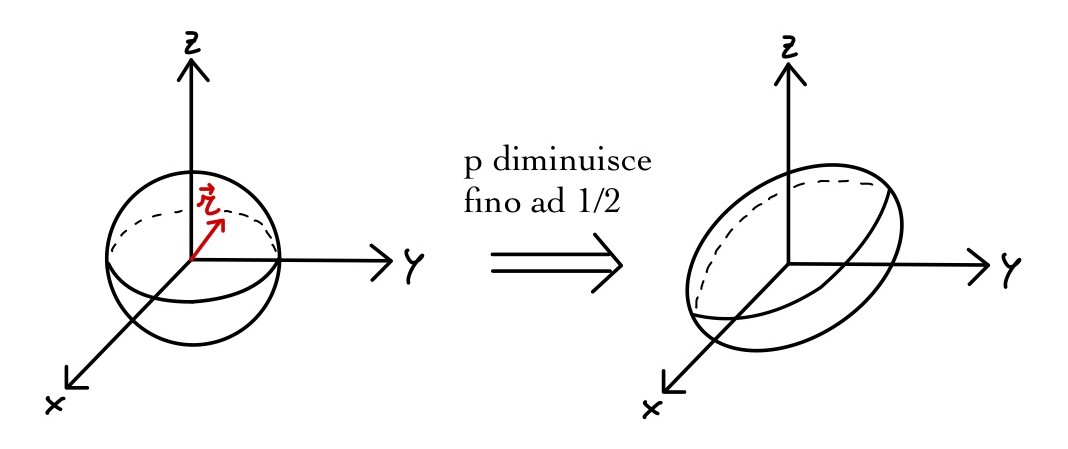
\includegraphics[scale=.37,keepaspectratio]{images/bit_flip_Bloch_1}} \quad
	\subfloat[][\text{Caso }$p=\frac{1}{2}$.\label{subfig:bit_flip_Bloch_2} ]{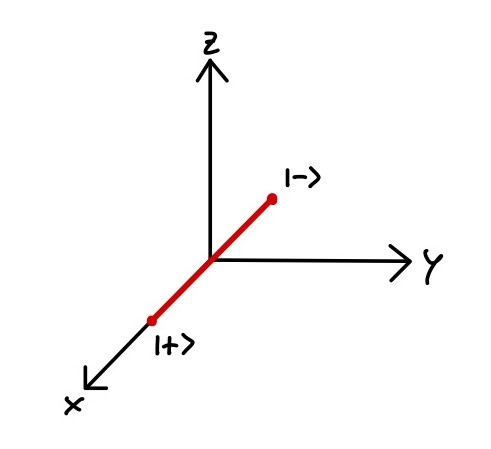
\includegraphics[scale=.37,keepaspectratio]{images/bit_flip_Bloch_2}}
	\caption{Cambiamento della sfera di Bloch nel bit flip channel al variare di $p$.}
    \label{fig:bit_flip_Bloch}
    \end{figure}
    \noindent Notiamo che, viceversa, al diminuire di $p$ con $0 \leq p \leq \frac{1}{2}$ la sfera di Bloch ritorna ad essere un ellissoide: passa dall'essere il segmento di Figura \ref{subfig:bit_flip_Bloch_2} fino alla sfera unitaria originale per $p= 0$. 
\end{esempio}


\begin{esempio}[\textbf{Phase flip channel}]\label{es:phase_flip}
    Si tratta del caso analogo all'esempio precedente in cui $X$ è sostituita da $Z$. In questa situazione sappiamo che $Z$ agisce come $a \ket{0} + b \ket{1} \rightarrow a \ket{0} - b \ket{1}$ (si ricordi che $-1 = e^{i \pi}$), quindi cambia la fase relativa tra gli stati (importante per fenomeni di interferenza). In questo caso gli operatori $E_k$ sono
    \begin{equation*}
        E_0 = \sqrt{p} \, \mathbb{I} = \sqrt{p}
        \begin{pmatrix}
            1 & 0 \\ 0 & 1
        \end{pmatrix} \, , \qquad
        E_1 = \sqrt{1-p} Z = \sqrt{1-p}
        \begin{pmatrix}
            1 & 0 \\ 0 & -1
        \end{pmatrix} \, ;
    \end{equation*}
    dove analogamente $1-p$ ha l'interpretazione della probabilità che lo stato possa subire un cambio di fase. Come nell'esempio precedente la trasformazione di $\rho$ sarà
    \begin{align*}
        \rho \rightarrow \sum_k E_k \rho E_k^\dag &= E_0 \rho E_0^\dag + E_1 \rho E_1^\dag = p \frac{\mathbb{I} + \vec{r} \cdot \vec{\sigma}}{2} + (1-p) Z \frac{\mathbb{I} + \vec{r} \cdot \vec{\sigma}}{2} Z \\
        &= p \frac{\mathbb{I} + r_1 \sigma_1 + r_2 \sigma_2 + r_3 \sigma_3}{2} + (1-p) \frac{\mathbb{I} - r_1 \sigma_1 - r_2 \sigma_2 + r_3 \sigma_3}{2} \\
        &= \frac{\mathbb{I} + r_3 \sigma_3 + (2p-1) r_1 \sigma_1 + (2p-1) r_2 \sigma_2}{2} \equiv \mathcal{E}(\rho) \, ;
    \end{align*}
    perciò in termini della sfera di Bloch avremo
    \begin{equation*}
        (r_1,r_2,r_3) \rightarrow \left[ (2p-1) r_1, (2p-1)r_2, r_3 \right] \, .
    \end{equation*}
    Le situazioni sono mostrate in Figura \ref{fig:phase_flip_Bloch}. Il caso è simile al precedente esempio, tuttavia l'ellissoide risulta questa volta schiacciato lungo $y$ e $x$ mantenendo $z$ costante. Quando $p = \frac{1}{2}$ la sfera collassa ad un segmento lungo $z$: a seconda del valore di $r_3$ lo stato corrisponde ad una miscela classica di $\ket{0}$ e $\ket{1}$. 
    \begin{figure}[!ht]
	\centering	
	\subfloat[][\text{La sfera di Bloch è un ellissoide per }$\frac{1}{2} \leq p \leq 1$.\label{subfig:phase_flip_Bloch_1} ]{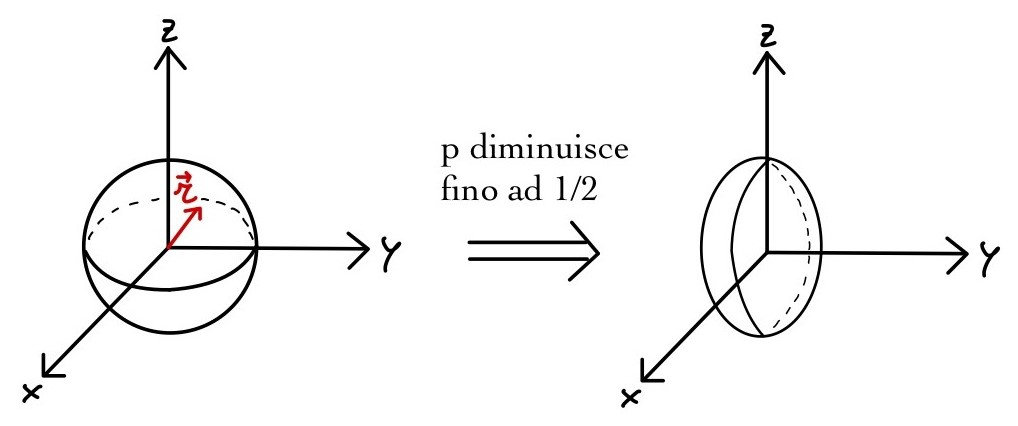
\includegraphics[scale=.37,keepaspectratio]{images/phase_flip_Bloch_1}} \quad
	\subfloat[][\text{Caso }$p=\frac{1}{2}$.\label{subfig:phase_flip_Bloch_2} ]{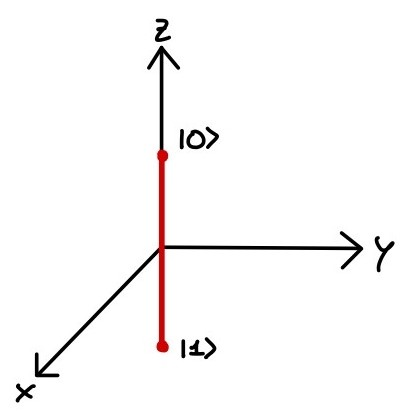
\includegraphics[scale=.37,keepaspectratio]{images/phase_flip_Bloch_2}}
	\caption{Cambiamento della sfera di Bloch nel phase flip channel al variare di $p$.}
    \label{fig:phase_flip_Bloch}
    \end{figure}
    
    \noindent Esplicitamente per $p = \frac{1}{2}$ avremo
    \begin{equation*}
        \mathcal{E}(\rho) = \frac{\mathbb{I}+ \sigma_3 r_3}{2} = 
        \begin{pmatrix}
            \frac{1+r_3}{2} & 0 \\ 0 & \frac{1-r_3}{2}
        \end{pmatrix}
        = \frac{1+r_3}{2} \ketbra{0} + \frac{1-r_3}{2} \ketbra{1} \, .
    \end{equation*}
    Notiamo che questo fenomeno accade anche quando si parte da uno stato puro: se si partisse dallo stato $\ket{+}$ (intersezione della sfera di Bloch con l'asse positivo delle $x$), allora esso sarebbe spinto, al diminuire di $p$, verso l'origine fino a quando $\rho = \frac{\mathbb{I}}{2}$.
\end{esempio}

\noindent Il cambiamento della fase relativa a seguito dell'interazione con l'ambiente è correlato al fenomeno (lo analizzeremo in dettaglio più avanti) che va sotto il nome di \textbf{decoerenza}. Per capire di che cosa si tratta supponiamo di partire con lo stato puro $\ket{\psi}$, dato dalla sovrapposizione generica $\ket{\psi} = a \ket{0} + b \ket{1}$. In termini di $\rho$ abbiamo visto che
\begin{equation*}
    \rho = \ketbra{\psi} =
    \begin{pmatrix}
        a \\ b
    \end{pmatrix}
    \otimes \begin{pmatrix} a^\ast & b^\ast \end{pmatrix} =
    \begin{pmatrix}
        \abs{a}^2 & a b^\ast \\ a^\ast b& \abs{b}^2
    \end{pmatrix} \, ;
\end{equation*}
i termini non diagonali misurano la sovrapposizione degli stati $\ket{0}$ e $\ket{1}$, quindi hanno a che fare con la fase relativa dello stato. Se si aspetta un tempo sufficientemente lungo, il qubit interagirà con l'ambiente tramite i phase flip channel producendo la seguente matrice diagonale:
\begin{equation*}
    \rho = 
    \begin{pmatrix}
        \abs{a}^2 & a b^\ast \\ a^\ast b& \abs{b}^2
    \end{pmatrix}
    \rightarrow
    \mathcal{E}(\rho) =
    \begin{pmatrix}
        (\ldots) & 0 \\ 0 & (\ldots)
    \end{pmatrix} \, ;
\end{equation*}
si ottiene quindi una miscela di stati (non è più uno stato puro) in cui tutte le informazioni legate alle fasi relative (termini non-diagonali) vengono perse! Questo fenomeno è la \textbf{decoerenza}: l'interazione con l'ambiente tramite phase flip channel tende a sopprimere tutti i termini non-diagonali di $\rho$. 

\begin{esempio}[\textbf{Bit-phase flip channel}]
    Ricordando che $XZ = -i Y$, se combiniamo il bit flip channel con il phase flip channel possiamo scrivere l'interazione con l'ambiente dovuta ai seguenti operatori
    \begin{equation*}
        E_0 = \sqrt{p} \, \mathbb{I} = \sqrt{p}
        \begin{pmatrix}
            1 & 0 \\ 0 & 1
        \end{pmatrix} \, , \qquad
        E_1 = \sqrt{1-p} Y = \sqrt{1-p}
        \begin{pmatrix}
            0 & -i \\ i & 0
        \end{pmatrix} \, ;
    \end{equation*}
    la trasformazione di $\rho$ non è altro che
    \begin{align*}
        \rho \rightarrow \sum_k E_k \rho E_k^\dag &= E_0 \rho E_0^\dag + E_1 \rho E_1^\dag = p \frac{\mathbb{I} + \vec{r} \cdot \vec{\sigma}}{2} + (1-p) Y \frac{\mathbb{I} + \vec{r} \cdot \vec{\sigma}}{2} Y \\
        &= p \frac{\mathbb{I} + r_1 \sigma_1 + r_2 \sigma_2 + r_3 \sigma_3}{2} + (1-p) \frac{\mathbb{I} - r_1 \sigma_1 + r_2 \sigma_2 - r_3 \sigma_3}{2} \\
        &= \frac{\mathbb{I} + r_2 \sigma_2 + (2p-1) r_1 \sigma_1 + (2p-1) r_3 \sigma_3}{2} \equiv \mathcal{E}(\rho) \, ;
    \end{align*}
    e quindi la sfera di Bloch si modifica come in Figura \ref{fig:bit_phase_flip_Bloch}. 
    \begin{figure}[!ht]
	\centering	
	\subfloat[][\text{La sfera di Bloch è un ellissoide per }$\frac{1}{2} \leq p \leq 1$.\label{subfig:bit_phase_flip_Bloch_1} ]{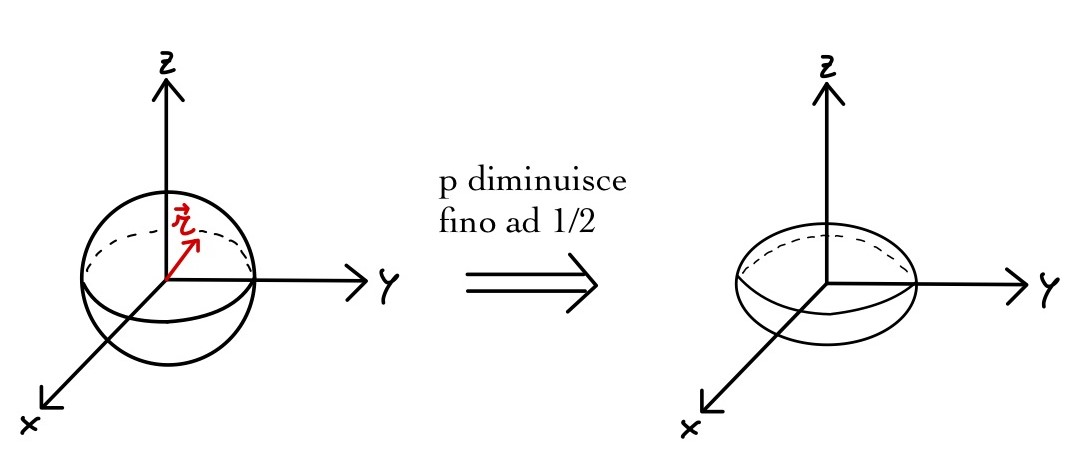
\includegraphics[scale=.37,keepaspectratio]{images/bit_phase_flip_Bloch_1}} \quad
	\subfloat[][\text{Caso }$p=\frac{1}{2}$.\label{subfig:bit_phase_flip_Bloch_2} ]{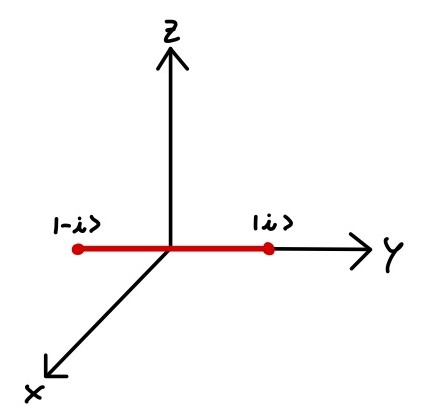
\includegraphics[scale=.37,keepaspectratio]{images/bit_phase_flip_Bloch_2}}
	\caption{Cambiamento della sfera di Bloch nel bit phase flip channel al variare di $p$.}
    \label{fig:bit_phase_flip_Bloch}
    \end{figure}
\end{esempio}

\begin{esempio}[\textbf{Depolarizing channel}]
    Un altro possibile modo di interagire con l'ambiente porta al cosiddetto \textbf{canale di depolarizzazione} per il quale la matrice densità del qubit diventa
    \begin{equation}\label{rho_depolarizing_channel}
        \mathcal{E}(\rho) = (1-p) \rho + \frac{p}{3} \left( X \rho X + Y \rho Y + Z \rho Z \right) \, ,
    \end{equation}
    dove $\frac{p}{3}$ non è altro che la probabilità che l'ambiente interagisca tramite ognuno dei termini nella parentesi tonda. Se utilizziamo la formula 
    \begin{equation*}
        \frac{\mathbb{I}}{2} = \frac{\rho + X \rho X + Y \rho Y + Z \rho Z}{4} \, , \quad \forall \; \rho = \frac{\mathbb{I}+ \vec{r} \cdot \vec{\sigma}}{2} \, ,
    \end{equation*}
    la quale è facilmente dimostrabile con la proprietà $\sigma_i \sigma_j = i \varepsilon_{ijk} \sigma_k$ per $i \neq j$, allora la \eqref{rho_depolarizing_channel} può essere scritta come
    \begin{equation}
        \mathcal{E}(\rho) = \tilde p \frac{\mathbb{I}}{2} + (1 - \tilde p) \rho \, , \; \text{ con } \; \tilde p = \frac{4}{3} p \, .
    \end{equation}
    Quest'ultima formula asserisce che nel canale di depolarizzazione vi è una probabilità di $1-\tilde p$ che nulla accada a $\rho$ e una probabilità di $\tilde p$ che ci sia un improvviso salto da $\rho$ a $\frac{\mathbb{I}}{2}$, ossia alla situazione in cui lo stato è il più indeterminato o depolarizzato possibile. In termini di effetti sulla sfera di Bloch, la situazione è mostrata nella Figura \ref{fig:depolarizing_channel}: quando $\tilde p \to 1$ la sfera di Bloch viene "schiacciata" in tutte le 3 possibili direzioni fino a quando, per $\tilde p = 1$, collassa ad un punto nell'origine. 
    \begin{figure}[!ht]
	\centering	
	\subfloat[][\text{La sfera di Bloch si restringe per }$\tilde p \to 1$.\label{subfig:depolarizing_channel_1} ]{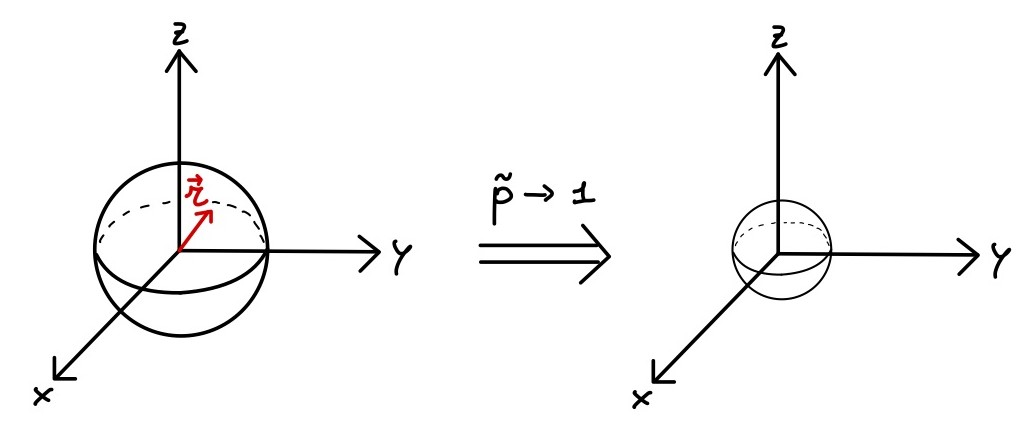
\includegraphics[scale=.37,keepaspectratio]{images/depolarizing_channel_1}} \quad
	\subfloat[][\text{Caso }$\tilde p = 1$.\label{subfig:depolarizing_channel_2} ]{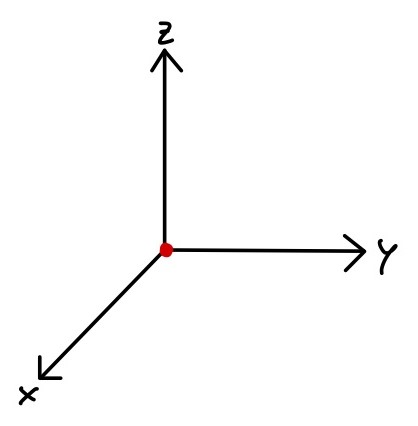
\includegraphics[scale=.37,keepaspectratio]{images/depolarizing_channel_2}}
	\caption{Cambiamento della sfera di Bloch nel canale di depolarizzazione al variare di $\tilde p$.}
    \label{fig:depolarizing_channel}
    \end{figure}
\end{esempio}

\noindent La caratterizzazione più completa dell'interazione dei qubit con l'ambiente è offerta dai fenomeni dell'\textbf{amplitude damping} ("smorzamento dell'ampiezza") e \textbf{phase damping} ("smorzamento della fase"): il primo è associato alla perdita di energia, tipicamente a seguito dell'emissione spontanea di fotoni, mentre il secondo è dovuto alla perdita di fase, a causa degli scattering (in realtà sono una sorta di diffusioni) con le particelle dell'ambiente (gli stati rimangono tali, $\ket{0} \to \ket{0}$ e $\ket{1} \to \ket{1}$). Cominciamo con l'analisi del primo dei due.

%\subsection{Amplitude damping}
%In questa situazione si ha una perdita di energia del qubit nell'ambiente causata dall'emissione spontanea di fotoni, a seguito della quale il valore assoluto dei coefficienti dello stato %diminuisce. La situazione schematica è la seguente: 
%\begin{center}
%    $
%        \begin{matrix}
%             \\
%             \\
%            \text{Emissione spontanea}: \\
%        \end{matrix}
%        $
%    \raisebox{1.2em}{
%        \mbox{
%            \Qcircuit @C=2em @R=2em {
%                & \qw & \rstick{\ket{1}} \qw \\
%                & \raisebox{.3em}{\begin{huge}$\downarrow$\end{huge}} & \raisebox{.05em}{\begin{huge} $\rightsquigarrow$ \end{huge}}\\
%                & \qw & \rstick{\ket{0}} \qw
%            }
%        }
%    }
%\end{center}
%\vspace{0.2cm}
%quindi se aspettiamo un tempo sufficientemente lungo il generico stato $a \ket{0} + b \ket{1}$ collassa in $\ket{0}$ a seguito di $\abs{b}^2 \to 0$. Possiamo descrivere la fisica %dell'emissione spontanea del fotone dal punto di vista dell'ambiente nel modo seguente: assumiamo che esso presenti due stati tali che
%\begin{align*}
%    \ket{0}_E &= \text{Nessuna emissione di fotoni}. \\
%    \ket{1}_E &= \text{1 fotone emesso}. 
%\end{align*}
%In questo modo il sistema totale $\mathcal{H}_q \otimes \mathcal{H}_E$ evolve con l'evoluzione unitaria $U$ tale che
%\begin{equation}\label{variazione_stati_emissione_spontanea}
%    U \, : \; 
%    \begin{cases}
%        \ket{0} \otimes \ket{0}_E &\rightarrow  \ket{0} \otimes \ket{0}_E \\
%        \ket{1} \otimes \ket{0}_E &\rightarrow  \sqrt{1-p} \ket{1} \otimes \ket{0}_E + \sqrt{p} \ket{0} \otimes \ket{1}_E
%    \end{cases} \, ,
%\end{equation}
%dove risulta evidente che $p$ è la probabilità in cui si abbia emissione spontanea, mentre $1-p$ è la probabilità che non accade nulla. Notiamo che le trasformazioni %\eqref{variazione_stati_emissione_spontanea} sono unitarie perché è immediato verificare che il prodotto scalare è conservato. Cosa succede quando calcoliamo la traccia parziale su %$\mathcal{H}_E$? Dobbiamo calcolare gli operation elements \eqref{E_k} dove $\ket{e_0} \equiv \ket{0}_E$ e $\ket{e_1} \equiv \ket{1}_E$. Dalla forma delle trasformazioni %\eqref{variazione_stati_emissione_spontanea} è facile vedere che hanno la seguente espressione:
%\begin{equation}\label{E_k_spontaneous_emission}
%    E_0 = 
%    \begin{pmatrix}
%        1 & 0 \\ 0 & \sqrt{1-p}
%    \end{pmatrix} \, , \qquad
%    E_1 =
%    \begin{pmatrix}
%        0 & \sqrt{p} \\ 0 & 0
%    \end{pmatrix} \, .
%\end{equation}